 \begin{figure}[H]
        \centering
        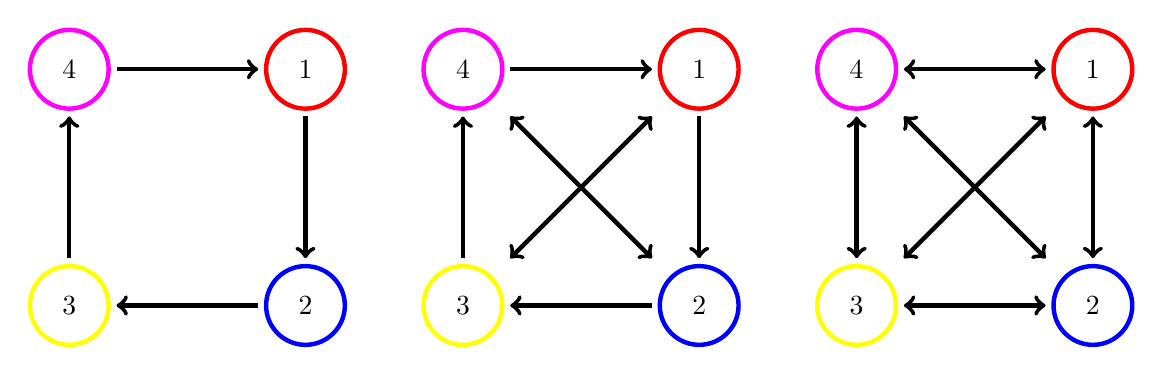
\begin{tikzpicture}
            \definecolor{cl1}{HTML}{FF0000}
            \definecolor{cl2}{HTML}{0000FF}
            \definecolor{cl3}{HTML}{FFFF00}
            \definecolor{cl4}{HTML}{FF00FF}
            \definecolor{cl5}{HTML}{00FFFF}
            \draw[ultra thick, draw=cl1] (+1.5,3) circle (0.5cm) node {$1$};
            \draw[ultra thick, draw=cl2] (+1.5,0) circle (0.5cm) node {$2$};
            \draw[ultra thick, draw=cl3] (-1.5,0) circle (0.5cm) node {$3$};
            \draw[ultra thick, draw=cl4] (-1.5,3) circle (0.5cm) node {$4$};
            \draw[ultra thick, ->] ( 1.5,2.4) -- ( 1.5,0.6);
            \draw[ultra thick, ->] ( 0.9,0.0) -- (-0.9,0.0);
            \draw[ultra thick, ->] (-1.5,0.6) -- (-1.5,2.4);
            \draw[ultra thick, ->] (-0.9,3.0) -- ( 0.9,3.0);
            \draw[ultra thick, draw=cl1] (6.5,3) circle (0.5cm) node {$1$};
            \draw[ultra thick, draw=cl2] (6.5,0) circle (0.5cm) node {$2$};
            \draw[ultra thick, draw=cl3] (3.5,0) circle (0.5cm) node {$3$};
            \draw[ultra thick, draw=cl4] (3.5,3) circle (0.5cm) node {$4$};
            \draw[ultra thick,  ->] (6.5,2.4) -- (6.5,0.6);
            \draw[ultra thick,  ->] (5.9,0.0) -- (4.1,0.0);
            \draw[ultra thick,  ->] (3.5,0.6) -- (3.5,2.4);
            \draw[ultra thick,  ->] (4.1,3.0) -- (5.9,3.0);
            \draw[ultra thick, <->] (4.1,2.4) -- (5.9,0.6);
            \draw[ultra thick, <->] (4.1,0.6) -- (5.9,2.4);
            \draw[ultra thick, draw=cl1] (11.5,3) circle (0.5cm) node {$1$};
            \draw[ultra thick, draw=cl2] (11.5,0) circle (0.5cm) node {$2$};
            \draw[ultra thick, draw=cl3] ( 8.5,0) circle (0.5cm) node {$3$};
            \draw[ultra thick, draw=cl4] ( 8.5,3) circle (0.5cm) node {$4$};
            \draw[ultra thick, <->] (11.5,2.4) -- (11.5,0.6);
            \draw[ultra thick, <->] (10.9,0.0) -- ( 9.1,0.0);
            \draw[ultra thick, <->] ( 8.5,0.6) -- ( 8.5,2.4);
            \draw[ultra thick, <->] ( 9.1,3.0) -- (10.9,3.0);
            \draw[ultra thick, <->] ( 9.1,2.4) -- (10.9,0.6);
            \draw[ultra thick, <->] ( 9.1,0.6) -- (10.9,2.4);
        \end{tikzpicture}
        \caption{\imgtabtitle Á esquerda tem-se a regra que se é induzido a utilizar como primeira regra; ao meio tem-se a regra e à direita que realmente foi adotada como primeira regra tem-se a segunda regra adotada para quando $\textstyle\mathcal{N}=4$.}
        \label{fig:rot4}
    \end{figure}